\documentclass{beamer}
\usetheme{AnnArbor}
\usecolortheme{beaver}
\usepackage{tikz}
\usepackage{color}
\usepackage{listings}

\lstset{language=Java,
  basicstyle=\footnotesize\ttfamily,
  keywordstyle=\footnotesize\color{blue}\ttfamily,
  commentstyle=\footnotesize\color{gray}\ttfamily,
}

\definecolor{darkred}{rgb}{0.8,0,0}

\setbeamercolor{title}{fg=white,bg=darkred!80!black}
\setbeamercolor{frametitle}{fg=darkred!80!black,bg=white}
%\setbeamercolor{section in head/foot}{fg=green,bg=yellow}
%\setbeamercolor{subsection in head/foot}{bg=white}
\begin{document}
\title{Advanced Java Debugging}   
\author{Andrej Podhradsky}
\date{February 8, 2016} 
%\logo{\includegraphics[height=1cm]{reddeer_logo.png}\vspace{220pt}}

\addtobeamertemplate{title page}{\center{DevConf 2016}}{}

%\addtobeamertemplate{frametitle}{}{
%\begin{tikzpicture}[remember picture,overlay]
%\node[anchor=north east,yshift=-8pt] at (current page.north east) {DevConf 2016};
%\end{tikzpicture}}

\frame{\titlepage} 

% \frame{\frametitle{Table of contents}\tableofcontents} 

\section{Motivation}

\subsection{What is debugging}
\begin{frame}[fragile]
\frametitle{What is debugging}
\begin{itemize}
\item process of finding and fixing bugs
\item example: NullPointerException at line 3
\vspace{0.2cm}
\begin{lstlisting}[numbers=left]
public User findUser(String nickname) {
  for (User user : this.users) {
    if (user.getNickname().equals(nickname)) {
      return user;
    }
  }
  return null;
}
\end{lstlisting}
\end{itemize}
\end{frame}


\subsection{First debug}
\begin{frame}[fragile]
\frametitle{Using sysout}
\begin{itemize}
\item there are 2 possibilities for npe
\vspace{0.2cm}
\begin{lstlisting}[numbers=left]
public User findUser(String nickname) {
  for (User user : this.users) {
    System.out.println("user=" + user);
    System.out.println("nickname=" + user.getNickname());
    if (user.getNickname().equals(nickname)) {
      return user;
    }
  }
  return null;
}
\end{lstlisting}
\end{itemize}
\end{frame}

\section{Prepare your environment}

\subsection{Prepare your environment}
\begin{frame}[fragile]
\frametitle{Prepare your environment}
\begin{itemize}
\item JDK 6+ (command java -version)
\\\url{www.oracle.com/technetwork/java/javase/downloads}
\item Maven 3.0.5+ (command mvn -v)
  \\\url{https://maven.apache.org/download.cgi}
\item Eclipse IDE for Java (or JavaEE) Developers
\\\url{http://www.eclipse.org/downloads}
\item FriendBook
  \\\url{https://github.com/apodhrad/devconf2016}
  \begin{lstlisting}
    cd friendbook
    mvn clean verify
  \end{lstlisting}
\end{itemize}
\end{frame}

\subsection{FriendBook}
\begin{frame}[fragile]
\frametitle{FriendBook}
\begin{center}
  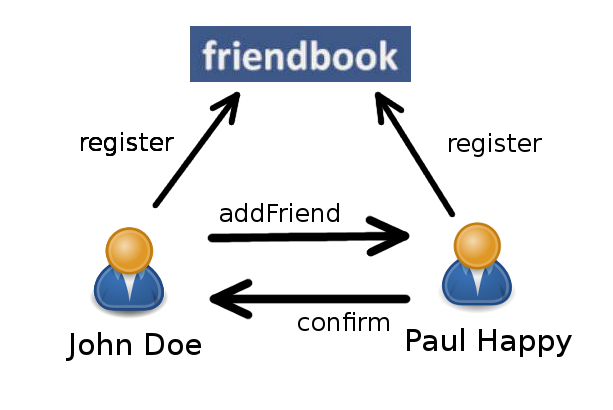
\includegraphics[width=11cm]{friendbook.png}
\end{center}  
\end{frame}


\section{Debugging}

\subsection{Pause and watch}
\begin{frame}[fragile]
\frametitle{Pause and watch}
Breakpoints can be set
\begin{itemize}
\item on a line with code
\item on an attribute
\item on a method
\item on a class
\item on an exception
\end{itemize}
Variables view
\begin{itemize}
\item watch all related variables
\item change a value of the variables
\end{itemize}
\end{frame}

\subsection{Pause when you want}
\begin{frame}[fragile]
\frametitle{Pause when you want}
\begin{itemize}
\item on access or modifification of the attribute
\item on entry or exit of the method
\item on your own condition
\end{itemize}
\end{frame}

\subsection{Watch what you want}
\begin{frame}[fragile]
\frametitle{Watch what you want}
\begin{itemize}
\item specify what you want to see by detail formatters
\item display and watch parts of the code
\item improve variables view by logical structure (e.g. HashMap)
\end{itemize}  
\end{frame}

\subsection{Jump to the frame}
\begin{frame}[fragile]
\frametitle{Jump to the frame}
\begin{itemize}
\item jump back in your stacktrace (frame)
\item cannot jump to native frame (or its successor like JUnit)
  \pause
\item to workaround this you can use test rule
\end{itemize}
\vspace{0.2cm}
\begin{lstlisting}
Statement apply(final Statement base, Description desc) {
  return new Statement() {
    @Override
    public void evaluate() throws Throwable {
      try {
        base.evaluate();
        "Breakpoint".toString();
      } catch (Throwable e) {
        throw e;
      }
    }
  };
}
\end{lstlisting}
\end{frame}

\subsection{Remote debugging}
\begin{frame}[fragile]
\frametitle{Remote debugging}
\begin{lstlisting}
java -Xdebug -Xnoagent -Djava.compiler=NONE \
-Xrunjdwp:transport=dt_socket,server=y,suspend=y,address=8001
\end{lstlisting}
\end{frame}

\section{Learning Materials}
\begin{frame}[fragile]
\frametitle{Learning Materials}
\begin{itemize}
\item Java Debugging with Eclipse - Tutorial\\\url{http://www.vogella.com/tutorials/EclipseDebugging/article.html}
\item Effective Java Debugging with Eclipse\\\url{http://eclipsesource.com/blogs/2013/01/08/effective-java-debugging-with-eclipse}
\item 10 Tips on Java Debugging with Eclipse\\\url{https://blog.codecentric.de/en/2013/04/again-10-tips-on-java-debugging-with-eclipse}
\end{itemize}
\end{frame}

\end{document}
